\documentclass[onecolumn, draftclsnofoot,10pt, compsoc]{IEEEtran}
\usepackage{graphicx}
\usepackage{url}
\usepackage{setspace}
\usepackage{outlines}

\usepackage{geometry}
\usepackage{mathtools}
\usepackage{graphicx}
\usepackage{epstopdf}
\usepackage{float}
\usepackage{longtable}

\geometry{textheight=9.5in, textwidth=7in}
\geometry{margin=0.75in}

% 1. Fill in these details
\def \CapstoneTeamName{		Team TriTone}
\def \CapstoneTeamNumber{		45}
\def \GroupMemberOne{			Aidan O'Malley}
\def \GroupMemberTwo{			Christopher Hebert}
\def \GroupMemberThree{			}
\def \CapstoneProjectName{		Music Theory Application}
\def \CapstoneSponsorPerson{		Lukas Hein}

% 2. Uncomment the appropriate line below so that the document type works
\def \DocType{		%Problem Statement
                %Requirements Document
                %Technology Review
                %Design Document
                Progress Report
                }
            
\newcommand{\NameSigPair}[1]{\par
\makebox[2.75in][r]{#1} \hfil 	\makebox[3.25in]{\makebox[2.25in]{\hrulefill} \hfill		\makebox[.75in]{\hrulefill}}
\par\vspace{-12pt} \textit{\tiny\noindent
\makebox[2.75in]{} \hfil		\makebox[3.25in]{\makebox[2.25in][r]{Signature} \hfill	\makebox[.75in][r]{Date}}}}
% 3. If the document is not to be signed, uncomment the RENEWcommand below
%\renewcommand{\NameSigPair}[1]{#1}

%%%%%%%%%%%%%%%%%%%%%%%%%%%%%%%%%%%%%%%
\begin{document}
\begin{titlepage}
    \pagenumbering{gobble}
    \begin{singlespace}
        % 
\includegraphics[height=4cm]{coe_v_spot1}
        \hfill 
        % 4. If you have a logo, use this includegraphics command to put it on the coversheet.
        %\includegraphics[height=4cm]{CompanyLogo}   
        \par\vspace{.2in}
        \centering
        \scshape{
            \huge CS Capstone \DocType \par
            {\large\today}\par
            \vspace{.5in}
            \textbf{\Huge\CapstoneProjectName}\par
            \vfill
            % {\large Prepared for}\par
            % \Huge \CapstoneSponsorCompany\par
            % \vspace{5pt}
            {\Large\NameSigPair{\CapstoneSponsorPerson}\par}
            {\large Prepared by }\par
            Group\CapstoneTeamNumber\par
            % 5. comment out the line below this one if you do not wish to name your team
            \CapstoneTeamName\par 
            \vspace{5pt}
            {\Large
                \NameSigPair{\GroupMemberOne}\par
                \NameSigPair{\GroupMemberTwo}\par
            }
            \vspace{20pt}
        }
        \begin{abstract}
        % 6. Fill in your abstract  
            This document is a progress report for Team TriTone containing information about what was accomplished over the first half of Spring term.
            There is a recap of the project as well as a summary individual progress, problems encountered, solutions, and where the project is headed from here.
        \end{abstract}     
    \end{singlespace}
\end{titlepage}
\newpage
\pagenumbering{arabic}
% \tableofcontents
% 7. uncomment this (if applicable). Consider adding a page break.
%\listoffigures
%\listoftables
% \clearpage

% 8. now you write!
\section{Project Recap}

Perfect Fifth is an iPhone and Android app aimed at teaching beginning composers the fundamentals of music theory in such a way that they can immediately apply the concepts toward creating their own music. 
The app presents the vision of music theory belonging to Lukas Hein, our client, which he calls the schedule of tonal gravity. 
It provides a simple foundation for choosing which chords resolve to each other using a tool known as the circle of fifths.

The main page of the Music Theory App is an interactive circle of fifths. The app also provides reference pages, for learning the fundamentals: including information about notes, intervals, keys, chords, and how to use the circle of fifths and tonal gravity to compose.
The app gives the musician a composition page that allows her to try composing phrases digitally, and have the app analyze the phrase according to tonal gravity theory.

\section{Where We Are}

\subsection{Circle of Fifths Page}

The first thing to notice about the Circle of Fifths is the brilliant pastel rainbow wheel.
The circle can be rotated by dragging in a circular motion to change the root tone of the key.
The circle can also be rotated by tapping on one of the notes in the sidebar.

\begin{center}
\includegraphics[width=0.25\textwidth]{major-circle}
\end{center}

The Circle of Fifths can show or hide parallel and relative keys.
The buttons for this are text only, and the text changes depending on the current state.
For example, when parallel key is shown, the "Hide Parallel" button is visible.
When "Hide Parallel" is tapped, the parallel key's qualities are now hidden, and the text displays "Show Parallel".

A third toggle switches the current key between major and minor.

\begin{center}
\includegraphics[width=0.25\textwidth]{minor-circle}
\end{center}

There is a vertical bar to demonstrate the order of tonal gravity.
This bar can be scrolled up and down to see all of the tones, ordered by fifths.
The tones that are part of the current key are in a dark gray box in pastel colors associated with the circle.
Tapping on a note will change the key, and rotate the circle.

The horizontal bar contains all of the diatonic chords in the selected scale.
Any of the chords can be tapped to cause a modal to pop up that allows the user to view the notes that belong to that chord.

\begin{center}
\includegraphics[width=0.25\textwidth]{modal}
\end{center}

The modal can be dismissed by sliding down or tapping the "Hide me" text.

\subsection{Composition Page}

The composition page allows the user to compose a chord sequence.
It automatically performs several analyses on the chord sequence, as the user enters chord, and whenever the user changes the key.

The sets the key using the first set of radio buttons.
They can set the note name (A-G), the accidentals (flat, sharp, etc.), and whether the key is major or minor.

Similarly, they can create a chord, but instead of just choosing major or minor for chord quality, they can also select dominant or diminished.
Once they are ready to add their chord, they can press the "Add Chord" button.

If they want to start over, they can press "New Composition".

\begin{center}
\includegraphics[width=0.25\textwidth]{composition-1}
\end{center}

Tonal gravity analysis is performed between two chords.
It is indicated using an arrow or a similar to sign.
A double arrow indicates a leap, a single arrow indicates a step, and a similarity sign indicates parallel motion.
Leap downs are drawn in red, since they are generally discouraged by the theory.
The rest of the transitions are in black.

\begin{center}
\includegraphics[width=0.25\textwidth]{composition-4}
\end{center}

If a chord is a diatonic chord, it is displayed using the same pastel colors as found on the Circle of Fifths.

\begin{center}
\includegraphics[width=0.25\textwidth]{composition-3}
\end{center}

If a chord is a substitute for a diatonic chord, or a borrowed chord, it is also shown in the same color as its diatonic functional equivalent.
If a chord's function is unknown it is shown in white.

A chord's function may change depending on what chords come after it.
It will be re-analyzed any time the user makes a change to the composition.

\begin{center}
\includegraphics[width=0.25\textwidth]{composition-2}
\end{center}

\subsection{Reference Pages}

The main sidebar menu now contains a table of contents, per results from our user studies.

\begin{center}
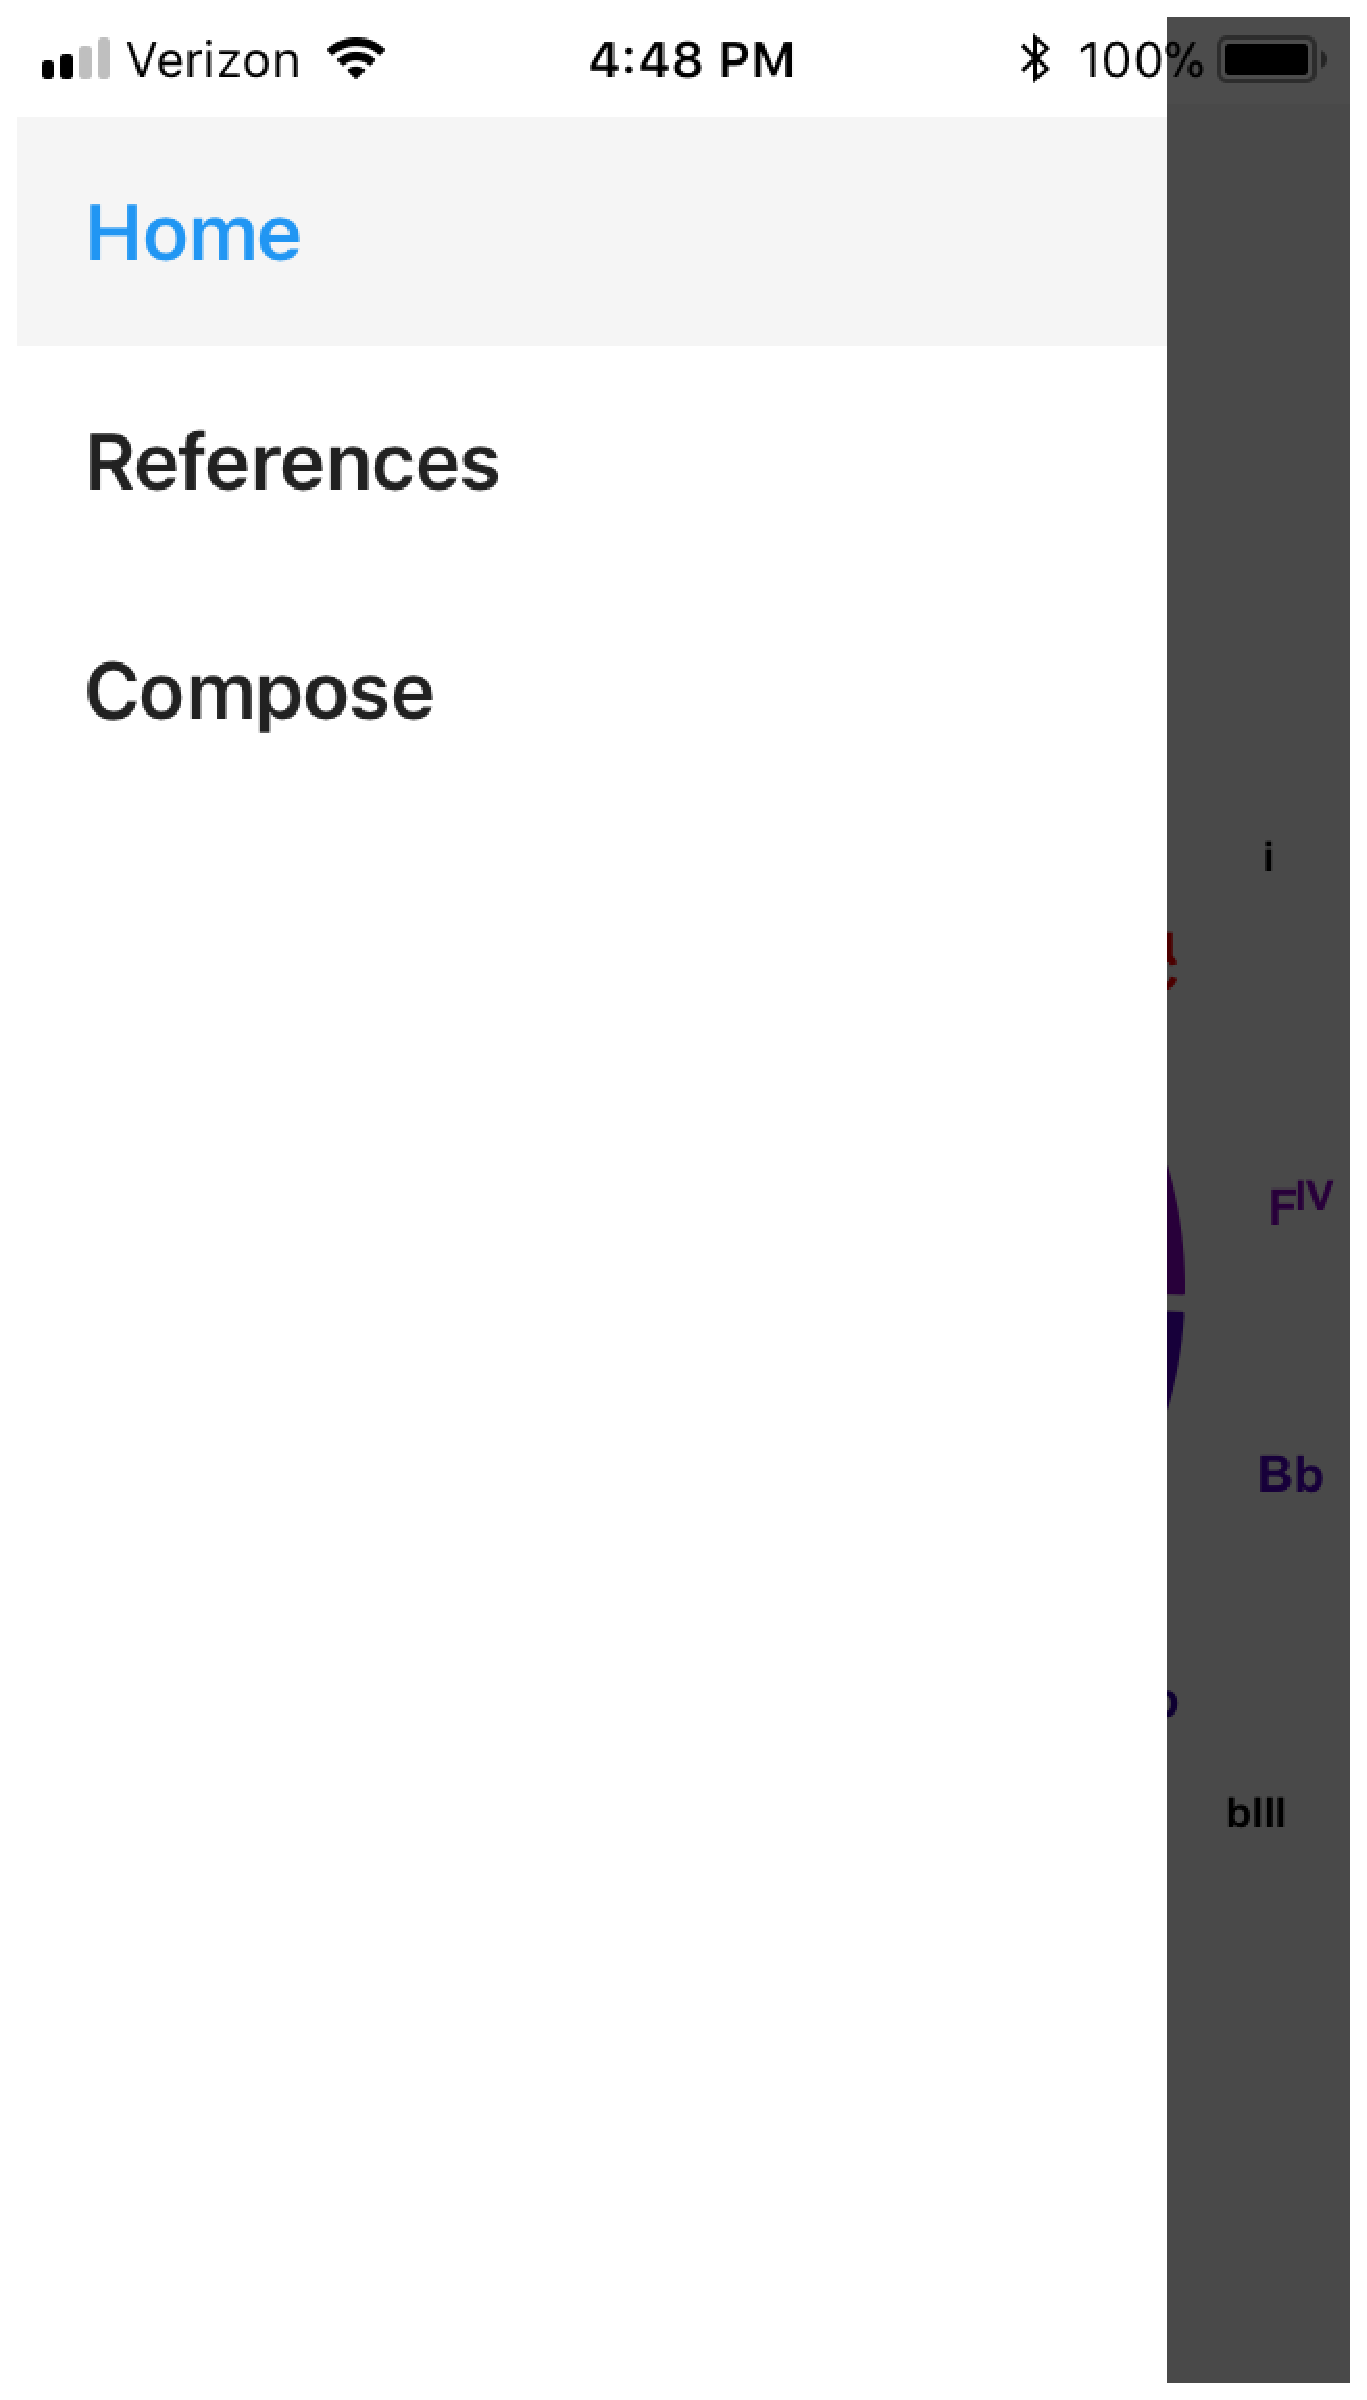
\includegraphics[width=0.25\textwidth]{menu}
\end{center}

Users can access any reference page from the table of contents, or they can swipe left and right through the pages.
Additionally, all pages, including the Circle of Fifths and Composition page, now have a Menu button to open the main sidebar menu, as well as a title.
This was also implemented as a direct result of user confusion during our user studies.

\begin{center}
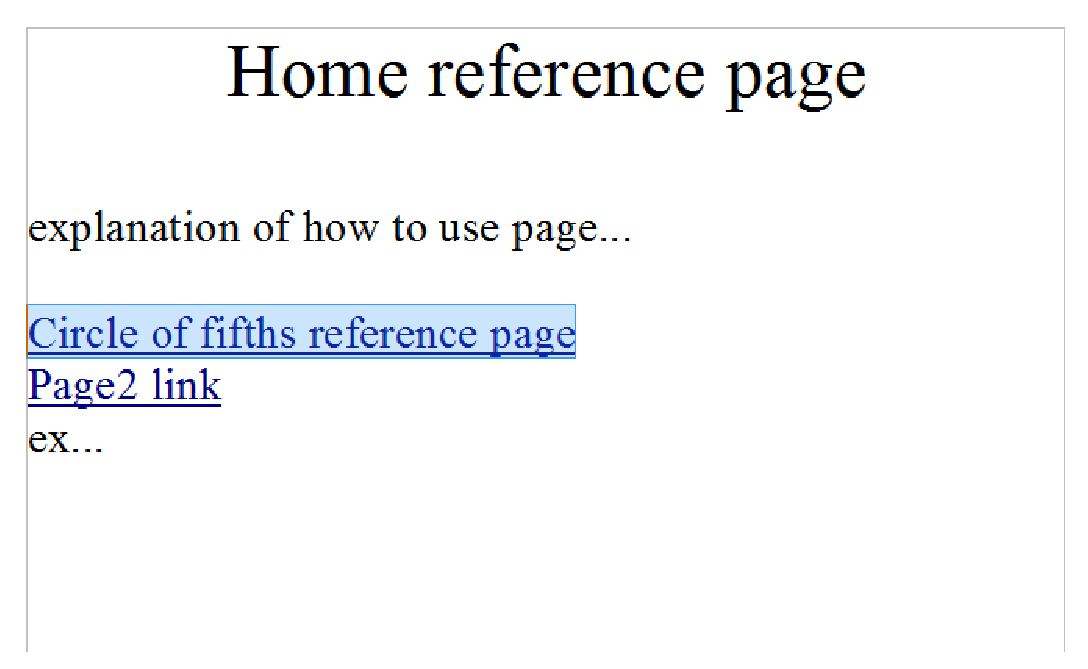
\includegraphics[width=0.25\textwidth]{references}
\end{center}

\section{Changes Made This Term}
\subsection{Aidan}
\begin{outline}
\1 Added jest for integration testing
\2 added integration tests for the Circle of Fifths algorithms.
\1 Created reference pages
\2 Created a style file to keep consistent between these pages.
\1 Created app icon for use in the various app stores
\begin{center}
\includegraphics[width=0.25\textwidth]{icon}
\end{center}

\1 Refactored Circle of Fifths
\2 Initially I was building up a scale based on the current key, then the fifth notes around the circle were built off of that scale, then using the fifths and the root note, I decided where the qualities for the current key, parallel, and relative keys would be placed. After using the application more and more I discovered that this was unnecessarily complex.
\2 Turns out, the qualities actually stay in the same position around the circle. These qualities only change locations when switching between major and minor scales but relative, parallel, and current key qualities stay in the same place for every major key and the same can be said for every minor key.
\2 It also turns out that the fifths around the circle stays the same for the same note, even if the scale changes.
\2 The new implementation now computes the fifths for a specific note. The current key, relative key, and parallel key text is now determined with two arrays of text for both major and minor keys. If the current scale is major, we select the major array for each of these key options and vice versa if the current scale is minor. This implementation is now easier to test and to expand upon in future application updates.

\end{outline}
\subsection{Christopher}
This term I:
\begin{outline}
\1 added analysis of chords, including analysis of:
\2 borrowed chords
\2 diatonic chords
\2 tritone substitutes
\2 secondary dominants
\1 added coloring to analyzed chords.
\1 added coloring to tonal gravity changes: red for leap down, and black for everything else.
\1 added V chord as alternative to V7.
\1 added tests for algorithms.
\1 added Menu button and title bar to all pages.
\1 added comments to document all of the code I had written.
\1 added documentation in README.
\1 added tritone reference page.
\1 added table of contents for reference pages.
\end{outline}

\section{What Is Left To Do}
We still need to upload the app to the iOS app store and to the Google Play store.
From our user studies, we decided it would be a good idea to add a tutorial overlay.
This overlay would appear on the first usage of the app.
It would show what buttons do what, what is interact-able, and where to start learning.
We also have several more stretch goals that we can work on:

\begin{itemize}
\item Create a Tutorial Overlay.
\item Add persistent state for Composition Page.
\item Link state of Composition Page Key to Circle of Fifths Page.
\item Remove the sidebar from the Circle of Fifths.
\item Move the diatonic chords to the side.
\item Add hyper-links in Reference pages.
\item Separate colors for Major and Minor keys.
\item Colors should match for Composition and Circle of Fifths pages.
\end{itemize}

\section{What Has Impeded our Progress, and Our Solutions}

\begin{outline}
\1 Challenge: Choosing colors for the rainbow which are easily visible on a single background.
	\2	Solution: Use pastel colors.
\1 Challenge: Creating a title bar and menu button for all pages.
	\2 Solution: Wrap each page in a Stack Navigation element with a title and button which opens the menu.
\1 Challenge: Determine if a chord is a tritone substitute, or just a weird chord.
	\2 Solution: Look at the next chord to see if its root is a half step down.
\end{outline}

\section{User Study}
Our application is pretty understandable in implementation and follows a lot of industry standards such as a navigation bar with titles for each page and a sidebar menu that swipes out from the left. However, these necessary navigation options weren't available to a user until after analyzing our user study's results. Before beginning any studies, we compiled a list of tasks for a user to go through to determine whether our interface was usable:

\begin{outline}
\1 Navigate to the composition page.
\1 Navigate to the reference pages.
\1 Change the root note in the home page in two different ways.
\1 Toggle the parallel key.
\1 Toggle the relative key.
\1 Change the scale quality.
\1 Create a composition in the key of F major with chords 'Fmaj Bbmaj C7'.
\end{outline}

We found that a few of these tasks were difficult for the user to accompish without assistance. This was clearly due to a lack of visibility of all of a user's options. The user was easily able to complete every interaction necessary on the circle of fifths home page and the composition page, however, the navigation tasks were very hard for the user until they realized that the menu swiped out from the left. To solve this issue, we added a navigation bar with page titles and also a menu button. These updates solved the navigation troubles in subsequent user studies.

\section{Conclusion}

The team dynamic has been good.
Lukas has been a good client to work with.
He has been very reasonable, clear, and level-headed about his requests.
Aidan and Christopher are both considering continuing work on the app during the summer.
Although we have encountered problems, we have been able to work through them, or push them aside until we know enough to work through them.
We both feel ready for expo, and ready to release the app to the iOS and Google Play stores.

\end{document}